\chapter{Capacidade de Armazenamento}

Vimos que a geometria do disco rígido envolve trilhas, setores e cilindros e que em cada setor do disco cabem 512 bytes de informação. Para identificar a capacidade de armazenamento de um disco basta utilizar a geometria, se um disco tem 2.448 cilindros, 16 lados (ou ``cabeças'' de leitura) e 63 setores por trilha, terá 2.448 x 16 x 63 = 2.467.584 setores. Logo, se multiplicarmos a quantidade de setores pela quantidade de informação que cabe em cada setor teremos a capacidade total do disco, que no caso é de 1.263.403.008 bytes, e como cada KB tem 1.024 bytes, dividindo-se por 1.024 uma vez para identificar a quantidade de KB do disco, divide-se novamente para identificar a quantidade em MB e novamente para identificar a quantidade em GB. Sendo assim esse disco teria a capacidade real de 1.18 GB.

\chapter{FAT}

\section{FAT-16}

O sistema FAT (File Allocation Table), utiliza uma tabela de alocação de arquivos representando um mapa de utilização do disco, o que permite ao sistema operacional ser capaz de saber exatamente onde um determinado arquivo está armazenado.

A FAT possui várias posições para localização de arquivos no disco. Como cada posição na FAT-16 utiliza 16 bits, podemos ter, no máximo, 256 (16 \^ 2) = 65.536 posições na FAT.

\subsection{Tabela de Alocação}

Como em um setor cabem 512 bytes, teoricamente, só poderiamos ter discos de 65.536 x 512 bytes = 33.554.432 bytes = 32 MB. Por esse motivo, o sistema FAT-16 não trabalha com setores mas sim com unidades de alocação chamadas \emph{\textbf{clusters}}, que é um conjunto de setores.

\subsection{Cluster}

Ao invés de cada posição da FAT apontar para um setor, ela aponta para um cluster, podendo ser de 1, 2, 4 ou mais setores do disco. O tamanho do cluster é definido automaticamente pelo sistema operacional quando o disco é formatado, seguindo uma tabela.

Sendo o cluster a menor unidade a ser acessada pelo sistema operacional, os arquivos deverão ter obrigatoriamente tamanhos múltiplos do tamanho do cluster, o que significa que um arquivo de 100 KB em um disco rígido que utilize clusters de 8KB obrigatoriamente ocupará 13 clusters e não 12,5 como seria a divisão de 100 por 8. Isso daria um total de 104 KB, neste caso temos um \emph{\textbf{desperdício}} de 4 KB. Quanto maior o tamanho do cluster, maior o desperdício.

Esse espaço deixado pelo arquivo dentro do cluster é muito importante para a forense computacional, chamado de \textbf{Slack Space}. Esse espaço costuma ficar vestígio de arquivos manipulados no sistema. 

\begin{citacao}
  Forense em sistemas FAT-16 podem apontar grandes quantidades de informações em slack space.
\end{citacao}

Todo o espaço que de armazenamento que sobra de um cluster não é reutilizado para armazenar outro arquivo. \emph{Um cluster só pode ser utilizado por um arquivo.}

Uma limitação do FAT-16 é que ele só permite gerenciar discos de até 2 GB de partição.

\subsection{FAT-32}

Com o FAT-32 o tamanho do cluster é sensivelmente menor, fazendo com que haja bem menos desperdício, reduzindo o slack space. Permite, também, o uso de discos maiores, até 1 TB em uma partição.

\section{NTFS}

Esse sistema de arquivos permite que a menor unidade de alocação (512 bytes) possa ser usada como o próprio setor, evitando assim desperdício de espaço.

O sistema NTFS utiliza 64 bits para endereçar os dados em sua MFT (Master File Table - tabela de endereçamento). Com o uso de clusters de 64 KB o limite de dados pode chegar aos 256 TB. O tamanho do cluster é definido automaticamente pelo sistema operacional ou pela formatação de uma partição, podendo ir de 512 bytes a 64 KB, e também podendo ser definido pelo usuário em procedimentos específicos.

\begin{citacao}
  Durante o processo de formatação do disco, é criado o MBR (Master Boot Record). O MBR contém uma quantidade pequena de códigos executáveis chamada de ``master boot code'' e contém também a tabela de partição do disco. A tabela de partição contém um determinado número de campos para descrever a partição. Um desses campos é o System ID, que define o file system, como o NTFS, na partição. Para volumes NTFS o ID é 0x07. 
\end{citacao}

A figura \ref{fig:ntfs} demonstra a arquitetura do NTFS.

\begin{figure}[htb]
	\centering
	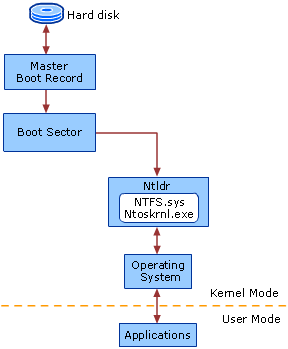
\includegraphics[width=0.8\textwidth]{sistemas_de_arquivos/fig/ntfs.png}
	\caption{Arquitetura do NTFS}
	\label{fig:ntfs}
\end{figure}

\newpage

O link \textbf{http://technet.microsoft.com/en-us/library/cc781134(v=ws.10).aspx} serve como referência para aprofundamento no NTFS.

\subsection{Tolerância a Falhas}

Para preservar os dados o NTFS utiliza um esquema de \emph{journaling}, um arquivo de log que indica falhas para posterior recuperação de dados. O log registra todas as ações que acontecem no sistema em relação aos arquivos. Quando um documento é criado, um espaço é alocado para ele, suas permissões são definidas, e assim por diante. Nesse meio tempo pode haver uma queda de energia e o espaço definido para o arquivo ser alocado, mas não utilizado. Quando o sistema operacional é reativado, ele consulta o arquivo de log para saber quais procedimentos não foram executados por completo e executa a ação correspondente para corrigir o problema.

\subsection{MFT - Master File Table}

A MFT tem praticamente a mesma finalidade da FAT, porém, funciona de uma forma diferente.

O MFT registra atributos de cada arquivo armazenado, consistindo em uma série de informações como por exemplo:

\begin{itemize}
	\item Nome do arquivo;
	\item Data da última modificação;
	\item Permissões; e
	\item Localização na unidade de armazenamento.
\end{itemize}

Cada entrada na MFT possui cerca de 2 KB, onde são armazenados o nome do arquivo e seus atributos, sobrando uma pequena área de dados que é usada para guardar o início do arquivo.

\begin{citacao}
  Em alguns casos, não é possível armazenar nem mesmo os atributos do arquivo, neste caso, os atributos são gravados em clusters no HD e na MFT ficam as entradas que apontam para os clusters.
\end{citacao}

\subsection{EFS}

O EFS é um recurso de criptografia permitindo uma maior proteção dos dados por criptografia utilizando chaves públicas. A principal vantagem é que o dono dos arquivos protegidos pode determinar quais usuários prodem acessá-los.

\subsection{Multiple Data Streams}

NTFS suporta multiplos streams de dados, onde o nome da stream identifica um atributo de dados novo no arquivo. O stream, então, é um conjunto exclusivo de atributos de arquivos. Os streams possuem atributos diferentes como bloqueio de arquivo e tamanho mas, possui \emph{\textbf{permissões comuns}}. 

Esse recurso permite gerenciar os dados com uma única unidade. Exemplo de um stream:

{
\raggedright
myfile.dat:stream2
}

Uma biblioteca de arquivos pode existir onde os arquivos são definidos como streams alternativos, como mostra o exemplo:

{
\raggedright
library:file1
:file2
:file3
}

Um arquivo pode estar associado a mais de uma aplicação ao mesmo tempo, assim como  Microsoft Word e Microsoft WordPad. Um exemplo da estrutura de arquivo que demonstra a associação múltipla a várias aplicações mas não múltiplos arquivos:

{
\raggedright
program:source_file
:doc_file
:object_file
:executable_file
}

Uma forma de criar um arquivo com stream alternativo:

{
\raggedright
echo text > program:source_file
more < program:source_file
}

\cite{
Um detalhe muito importante é que essa funcionalidade está presente somente no NTFS e é incompatível para o FAT, ou seja, se um disco com sistema de arquivo FAT receber a cópia de um arquivo NTFS os streams e outros atributos não suportados pelo FAT serão perdidos sem nenhum aviso.}

\subsection{Change Journal}

O Change Journal é usado pelo NTFS para prover um log persistente de todas alterações feitas em arquivos no volume. \textbf{Para cada volume}, o NTFS usa o change journal para rastrear informações sobre inclusão, remoção e modificação de arquivos.

fonte: \textbf{http://www.readability.com/articles/xhgmtysq}

\section{EXT3}

Possui o recurso de recuperação de falhas, o \emph{\textbf{Journaling}}. Isso poderia ser relevante para a forense pois alguns dados e metadados registrados na área de ``Journal'' do sistema podem significar alguma coisa em uma investigação, principalmente se utilizando o tipo de trabalho ``Journal''.

\subsection{Journaling}

O ext3 trabalha com 3 diferentes tipos de Journaling:

\begin{itemize}
	\item \textbf{Journal}: grava todas mudanças em sistema de arquivos. É o mais lento dos três modos, mas é o que apresenta maior capacidade de evitar perda de dados;
	\item \textbf{Ordered}: grava somente mudanças em arquivos \emph{metadata} (arquivos que guardam informações de outros arquivos), mas guarda as atualizações no arquivo de dados antes de fazer as mudanças associadas ao sistema de arquivos. Este é o Journaling padrão nos sistemas de arquivos ext3;
	\item \textbf{Writeback}: também só grava mudanças para o sistema de arquivo em \emph{metadata}, mas utiliza o processo de escrita do sistema de arquivos em uso para gravação. É o mais rápido de todos, mas o menos confiável.
\end{itemize}

\subsection{Inode}

Os dados do arquivo são armazenados em unidades chamadas de ``blocos''. Um arquivo também possui um ``inode''. Os blocos e os inodes podem são numerados sequencialmente porém, o inode possui uma sequência diferente da dos blocos. Uma entrada de diretório consiste do nome do arquivo e de um número de inode. O inode também armazena o local dos blocos de dados, como pode ser visto na figura \ref{fig:inode}.

\begin{figure}
	\centering
	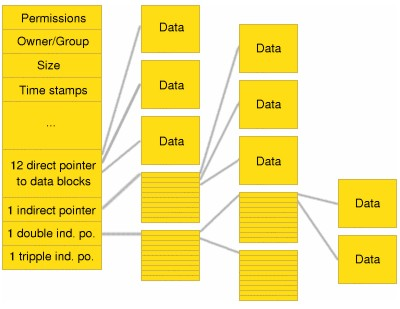
\includegraphics[width=0.8\textwidth]{sistemas_de_arquivos/fig/inode.jpg}
	\caption{Forma como o \emph{inode} armazena o local dos blocos de dados}
	\label{fig:inode}
\end{figure}

\begin{itemize}
	\item Os números dos primeiros 12 blocos são armazenados diretamente no inode - chamados de ``blocos diretos'' (pode ser visto na figura \ref{fig:inode} em ``12 direct pointer to data blocks'');
	\item O inode contém o número do bloco de um bloco indireto. (pode ser representado na figura \ref{fig:inode} em ``1 indirect pointer''). Um bloco indireto contém os números de blocos de 256 blocos de dados adicionais;
	\item O inode contém o número do bloco de um bloco duplamente indireto (pode ser visto na figura \ref{fig:inode} em ``1 double ind. po.''). Um bloco duplamente indireto contém os números de blocos de 256 blocos indiretos adicionais; e
	\item O inode contém o número do bloco de um bloco três vezes indireto. (pode ser visto na figura \ref{fig:inode} em ``1 tripple ind. po.''). Um bloco três vezes indireto contém os números de blocos de 256 blocos duplamente indiretos adicionais.
\end{itemize}

Sendo assim, o sistema de arquivo ext3 consiste de 5 componentes estruturais.

\begin{itemize}
	\item Células de armazenamento inode;
	\item Superblocos distribuídos;
	\item Mapa de blocos no sistema de arquivos;
	\item Resumo de emprego de blocos; e
	\item Conjunto de blocos de dados.
\end{itemize}

Cada partição de sistema de arquivos é dividida em grupos de blocos. Estruturas como as tabelas de inode são alocadas entre os grupos de blocos para que os blocos que são acessados juntos possam ser armazenados próximos uns dos outros no disco.

Inodes são entradas de tabelas de comprimento fixo, cada uma das quais armazenam informações sobre um arquivo existente no sistema de arquivos.

Os inodes são criados no momento da formatação lógica do hd. Assim é possível redimensionar o número de inodes de acordo com a capacidade do hd e o tipo e tamanho de arquivos que serão armazenados nele. O número de inodes não pode ser ajustado após a formatação inicial.

\subsection{Superbloco}

Registro que descreve as características do sistema de arquivos, conforme a figura \ref{fig:superbloco}.

\begin{figure}
	\centering
	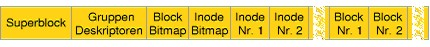
\includegraphics[width=0.8\textwidth]{sistemas_de_arquivos/fig/superbloco.jpg}
	\caption{Informações do superbloco}
	\label{fig:superbloco}
\end{figure}

O superbloco contém informações sobre:

\begin{itemize}
	\item Comprimento de um bloco de disco;
	\item Tamanho e localização das tabelas de inodes;
	\item Mapa de blocos de disco e informações sobre utilização; e
	\item Tamanho dos grupos de blocos.
\end{itemize}

O GNU/Linux mantém, para cada sistema de arquivos, um cópia do superbloco em memória RAM. A chamada de sistema ``sync'' despeja os dados sobre os superblocos que estão armazenados em memória cache para seus locais em disco, sincronizando as informações sobre o sistema de arquivos. Essa sincronização torna o sistema de arquivos consistente rapidamente. Essa operação acontece automaticamente em intervalos de 30s para sistemas ext2 e de 5s para sistemas ext3, reduzindo ainda mais a possibilidade de falhas em servidores com intensas atividades de gravação de arquivos.

\subsection{Mapa de Blocos}

É a tabela de blocos livres que o disco possui. Quando da gravação de um arquivo novo, esse mapa é verificado de modo que uma disposição eficiente seja utilizada.

\subsection{Resumos de Empregos de Blocos}

Registram informações básicas sobre os blocos que já se encontram em uso.

Até este ponto os sistemas ext2 e ext3 são idênticos.

\section{ReiserFS}

Possui suporte ao ``journaling'' e atualmente presente como padrão para distribuições GNU/Linux da SuSE, Gentoo e Linspire.

Ele trata toda a partição como se fosse uma única tabela de banco de dados contendo diretórios, arquivos e metadados dentro de uma mesma árvore. Essa característica exigiu o uso de técnicas de indexação mais complexas para tornar os tempos de resposta do ReiserFS mais eficientes comparados com outros sistemas de arquivos. O ReiserFS usa uma árvore \textbf{finita} (número de nós é limitado).

O ReiserFS possui suporte a arquivos maiores que 2GB.

ReiserFS usa árvores balanceadas (B*) para tornar o processo de busca de arquivos, informações sobre segurança e outros metadados mais eficientes.

Outra grande vantagem do ReiserFS é a alocação dinâmica de inodes, já que esse sistema de arquivos não os aloca em espaços fixos ou blocos e sim, aloca o tamanho exato que o arquivo precisa. Em sistemas baseados em inodes fixos, como o EXT3, o espaço no disco é alocado em blocos que variam de 512 a 4096 bytes ou até maior, caso o arquivo exceda um múltiplo exato do tamanho do bloco.

Seu uso de funções hash e árvores balanceadas (B*), ao invés de seqüências infindáveis de inodes, tornam a procura de um arquivo em uma dezena ou em uma grande quantidade uma operação bem rápida.

No caso de um desligamento incorreto do sistema, o ReiserFS é capaz de recuperar a consistência do sistema de arquivos em frações de segundo e a possibilidade de perda de pastas ou partições é nula. Em compensação, os arquivos que eventualmente estiverem sendo gravados no exato momento em que acabou a energia ficarão com seus dados alterados. Você continuará tendo acesso aos arquivos normalmente, mas o conteúdo estará truncado ou incompleto.

Fonte: \textbf{http://www.readability.com/articles/euug5xab}

